\documentclass{beamer}
\usepackage[utf8]{inputenc}

\usetheme{Madrid}
\usecolortheme{default}
\usepackage{amsmath,amssymb,amsfonts,amsthm}
\usepackage{txfonts}
\usepackage{tkz-euclide}
\usepackage{listings}
\usepackage{adjustbox}
\usepackage{array}
\usepackage{tabularx}
\usepackage{gvv}
\usepackage{lmodern}
\usepackage{circuitikz}
\usepackage{tikz}
\usepackage{graphicx}
\usepackage{multicol}

\setbeamertemplate{page number in head/foot}[totalframenumber]

\usepackage{tcolorbox}
\tcbuselibrary{minted,breakable,xparse,skins}



\definecolor{bg}{gray}{0.95}
\DeclareTCBListing{mintedbox}{O{}m!O{}}{%
  breakable=true,
  listing engine=minted,
  listing only,
  minted language=#2,
  minted style=default,
  minted options={%
    linenos,
    gobble=0,
    breaklines=true,
    breakafter=,,
    fontsize=\small,
    numbersep=8pt,
    #1},
  boxsep=0pt,
  left skip=0pt,
  right skip=0pt,
  left=25pt,
  right=0pt,
  top=3pt,
  bottom=3pt,
  arc=5pt,
  leftrule=0pt,
  rightrule=0pt,
  bottomrule=2pt,
  toprule=2pt,
  colback=bg,
  colframe=orange!70,
  enhanced,
  overlay={%
    \begin{tcbclipinterior}
    \fill[orange!20!white] (frame.south west) rectangle ([xshift=20pt]frame.north west);
    \end{tcbclipinterior}},
  #3,
}
\lstset{
    language=C,
    basicstyle=\ttfamily\small,
    keywordstyle=\color{blue},
    stringstyle=\color{orange},
    commentstyle=\color{green!60!black},
    numbers=left,
    numberstyle=\tiny\color{gray},
    breaklines=true,
    showstringspaces=false,
}
%------------------------------------------------------------
%This block of code defines the information to appear in the
%Title page
\title %optional
{4.13.34}
\date{September 30,2025}


\author 
{Jnanesh Sathisha karmar - EE25BTECH11029}



\begin{document}



\frame{\titlepage}
\begin{frame}Solve the following system of linear equations\\$x+2y-4=0$\\$2x+4y-12=0$\\

\end{frame}



\begin{frame}{Equation}
\textbf{Solution} Given details\\
\begin{align}
    x+2y-4=0\\
    2x+4y-12=0\\
    \myvec{1&2\\2&4}\myvec{x\\y}=\myvec{4\\12}\\
    \vec{A}\vec{x}=\vec{B}
\end{align}
\end{frame}
\begin{frame}{Theoretical Solution}
To determine if a unique solution exists, we calculate the determinant of the coefficient matrix

\begin{align}
    \det(\vec{A})=4-4=0
\end{align}
Since the determinant is zero, the matrix $\vec{A}$ is singular $\brak{\text{it has no inverse}}$. This means that the system does not have a unique solution. It will either have no solution or infinitely many solutions.\\
To find out which case it is, we use an augmented matrix $\augvec{1}{1}{\vec{A}&\vec{B}}$and apply row reduction.
\begin{align*}
    \augvec{2}{1}{1&2&4\\2&4&12}\xrightarrow{R_2 \rightarrow R_2-2R_1}\augvec{2}{1}{1&2&4\\0&0&4}
\end{align*}
\end{frame}
\begin{frame}{Theoretical Solution}
Since the second row of the reduced matrix corresponds to the equation $0x+0y=4$, which is a contradiction, the system is inconsistent and has no solution.
\end{frame}

\begin{frame}[fragile]
    \frametitle{C Code (1) - Function to store the points }

    \begin{lstlisting}
#include <stdio.h>
double get_y_for_line1(double x) {
    return (4.0 - x) / 2.0;
}

double get_y_for_line2(double x) {
    return (12.0 - 2.0 * x) / 4.0;
}

    \end{lstlisting}
\end{frame}

\begin{frame}[fragile]
    \frametitle{Python Code - Using Shared Object}
    \begin{lstlisting}
import ctypes
import numpy as np
import matplotlib.pyplot as plt

lib_path = './line_plotter.so'


line_lib = ctypes.CDLL(lib_path)


line_lib.get_y_for_line1.argtypes = [ctypes.c_double]
line_lib.get_y_for_line1.restype = ctypes.c_double

line_lib.get_y_for_line2.argtypes = [ctypes.c_double]
line_lib.get_y_for_line2.restype = ctypes.c_double
\end{lstlisting}
\end{frame}

\begin{frame}[fragile]
    \frametitle{Python Code - Using Shared Object}
    \begin{lstlisting}
x_values = np.linspace(-10, 10, 100)

y1_values = [line_lib.get_y_for_line1(x) for x in x_values]
y2_values = [line_lib.get_y_for_line2(x) for x in x_values]

plt.style.use('seaborn-v0_8-whitegrid')
plt.figure(figsize=(10, 8))

plt.plot(x_values, y1_values, label='x + 2y - 4 = 0', color='dodgerblue', linewidth=2)
plt.plot(x_values, y2_values, label='2x + 4y - 12 = 0', color='tomato', linewidth=2, linestyle='--')
\end{lstlisting}
\end{frame}
\begin{frame}[fragile]
    \frametitle{Python Code - Using Shared Object}
    \begin{lstlisting}
plt.title('Plot of Linear Equations', fontsize=16, fontweight='bold')
plt.xlabel('X-axis', fontsize=12)
plt.ylabel('Y-axis', fontsize=12)
plt.legend(fontsize=10)

plt.grid(True)
plt.axhline(0, color='black',linewidth=0.5)
plt.axvline(0, color='black',linewidth=0.5)
plt.axis('equal')
plt.savefig("./figs/lines.png") 
subprocess.run(shlex.split('termux-open ../figs/lines.png'))
plt.show()
\end{lstlisting}
\end{frame}


\begin{frame}{Plot-Using Both C and Python}
    \centering
    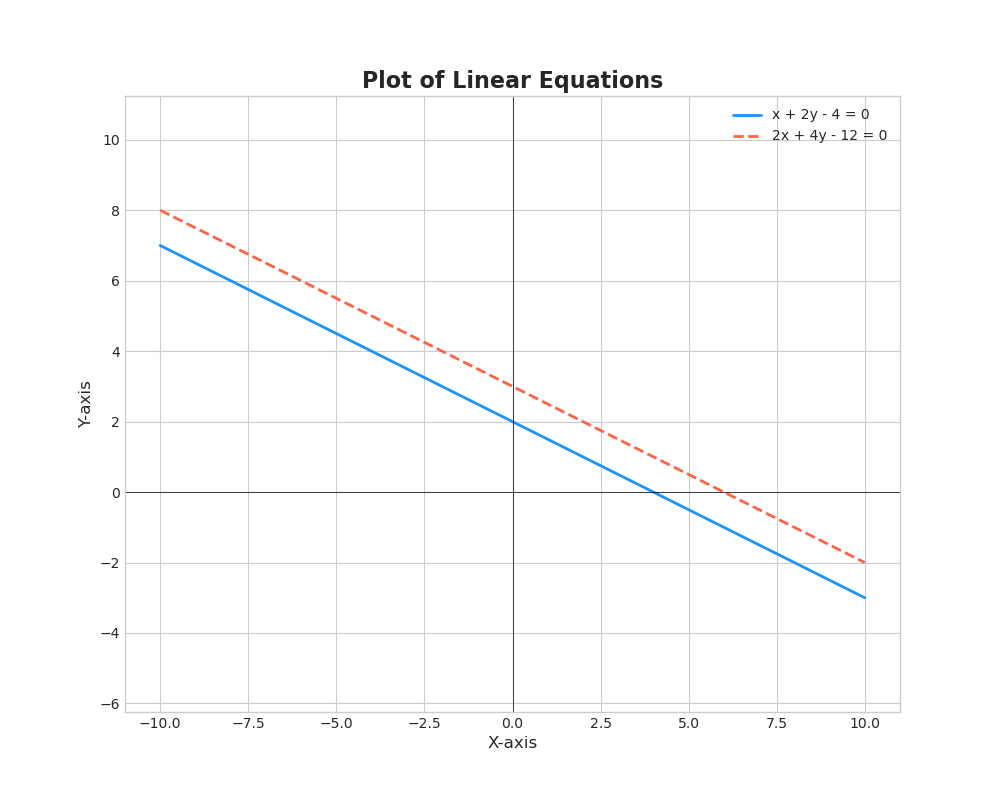
\includegraphics[width=\columnwidth, height=0.8\textheight, keepaspectratio]{figs/lines.png}     
\end{frame}

\begin{frame}[fragile]
    \frametitle{Python Code}
    \begin{lstlisting}
import numpy as np
import matplotlib.pyplot as plt

def get_y_for_line1(x):
    # Equation 1: x + 2y - 4 = 0  =>  y = (4 - x) / 2
    return (4 - x) / 2

def get_y_for_line2(x):
    # Equation 2: 2x + 4y - 12 = 0 =>  y = (12 - 2x) / 4
    return (12 - 2 * x) / 4

x_values = np.linspace(-10, 10, 100)

y1_values = get_y_for_line1(x_values)
y2_values = get_y_for_line2(x_values)
\end{lstlisting}
\end{frame}
\begin{frame}[fragile]
    \frametitle{Python Code}
    \begin{lstlisting}
plt.style.use('seaborn-v0_8-whitegrid')
plt.figure(figsize=(10, 8))
plt.plot(x_values, y1_values, label='x + 2y - 4 = 0', color='dodgerblue', linewidth=2)
plt.plot(x_values, y2_values, label='2x + 4y - 12 = 0', color='tomato', linewidth=2, linestyle='--')
plt.title('Plot of Linear Equations', fontsize=16, fontweight='bold')
plt.xlabel('X-axis', fontsize=12)
plt.ylabel('Y-axis', fontsize=12)
plt.legend(fontsize=10)
plt.savefig("./figs/lines2.png") 
plt.grid(True)
plt.axhline(0, color='black',linewidth=0.5)
plt.axvline(0, color='black',linewidth=0.5)
plt.axis('equal')

plt.show()
\end{lstlisting}
\end{frame}

\begin{frame}{Plot-Using only Python}
    \centering
    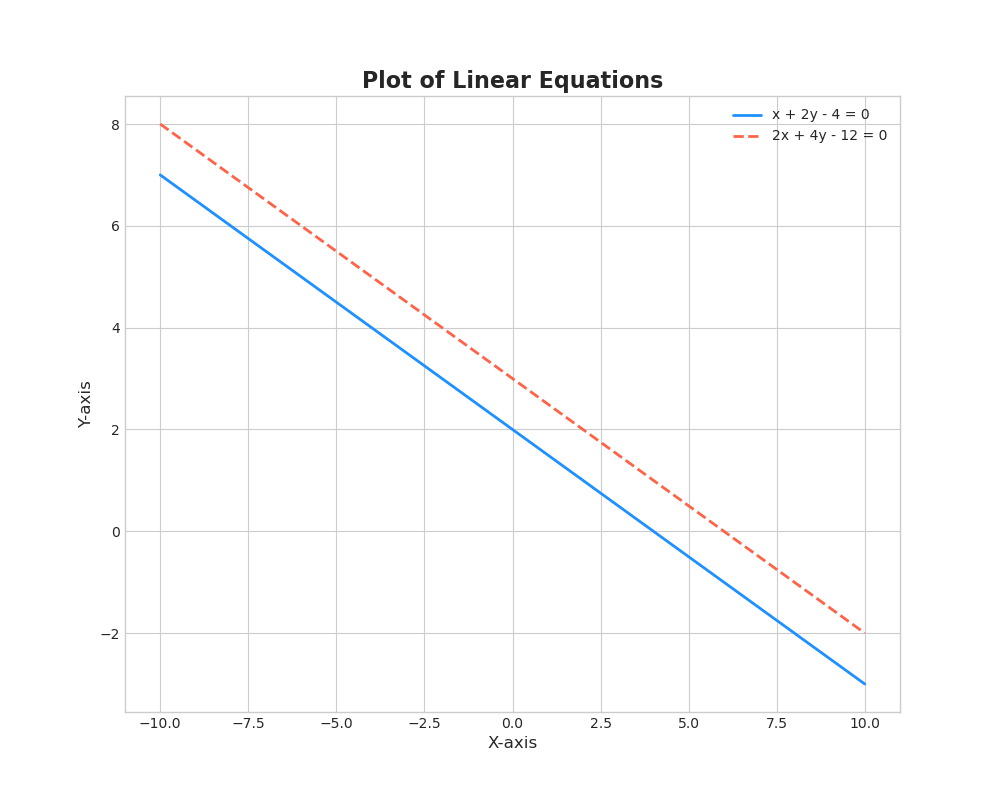
\includegraphics[width=\columnwidth, height=0.8\textheight, keepaspectratio]{figs/lines2.png}     
\end{frame}


\end{document}